\section{Experimental Results}
\label{sec:expResults}
%Results should be clearly displayed and should provide a suitable representation of your results for the points you wish to make. Graphs should be labeled in a legible font and if more than one result is displayed on the same graph then these should be clearly marked.   Please choose carefully rather than presenting every results. Too much information is hard to read and often hides the key information you wish to present. Make use of statistical methods when presenting results, where possible to strengthen the results.  Further, the format of the presentation of results should be chosen based on what issues in the results you wish to highlight. You may wish to present a subset in the experimental section and provide additional results in the appendix.

\subsection{Parameter Settings}
\label{subsec:parameterSettings_results}

Table \vref{table:parameterSettings2} shows the parameters tested, their candidate values and the selected value. The complete experimental steps with the corresponding results can be found in, Appendix \ref{appendixC}, Table \vref{table:pm1} and Table \vref{table:pm2}. 
    \begin{table}[H]
    \centering
    \begin{tabular}{|c|c||c|}
    \hline
    Parameters & Candidate values & Selected value\\
    \hline
    $s$ & 10, 25, 50, 100, 150 & 50$^*$ \\
    $i$ & 1, 10 , 50, 100, 125 & 100 \\
    $E$ & 1\%, 10\%, 25\% 50\%, 75\%, 90\%, 99\% & 50\% \\
    $p_{b}$ & 0.0, 0.1, 0.3, 0.5, 0.7, 0.9 & 0.9 \\
    $BR$ & 1\%, 10\%, 25\% 50\%, 75\%, 90\%, 99\% & 25\% \\
    $AF$ & 0\%, 1\%, 5\%, 10\%, 50\%, 75\%, 100\% & 25\% \\
    $CA$ & 0\%, 1\%, 5\%, 10\%, 50\%, 75\%, 100\% & 5\% \\
    \hline
    \end{tabular}
    \caption {Results from the parameter settings experiment}
    %The complete experimental steps with the corresponding results can be found in, Appendix \ref{appendixC}, Table \vref{table:pm1} and Table \vref{table:pm2}.
    \begin{itemize}[noitemsep]
    \item[$^*$:] \emph{\color{blue} Selected based on runtime}
    \end{itemize}
    \label{table:parameterSettings2}
    \end{table}


\subsection{Performance Comparison}
\label{subsec:performanceComparison_results}

%---------------------- Execution time ---------------------
\begin{table}[H]
    \centering
    \begin{tabular}{|l||l|l|l|l|l|l|}
    \hline
    Number of routes & Min & Avg & Median & Max & STD & RSD \\
    \hline
    4 & 491.0 & 555.2 & 553.0 & 644.0 & 31.0 & 5.59\%\\
    \hline
    \end{tabular}
    \caption {Executing time (in seconds) of SSO for route set designs with 4, }
   % 100 Monte Carlo runs
    \label{table:performanceComparison_ACOSSOBEST}
    \end{table}


%---------------------- ACO VS SSO ---------------------
    \begin{table}[H]
    \centering
    \begin{tabular}{|l||l|l|l|l|l|}
    \hline
    Algorithm & $d_0(\%)$ & $d_1(\%)$ & $d_2(\%)$ & $d_{unsat}(\%)$ & $ATT$ \\
    \hline
    ACO Best & 86.16 & 12.59 & 2.25 & 0.00 & 11.16 \\
    \hline
    SSO Best & 88.44 & 10.28 & 1.29 & 0.00 & 10.67 \\
    \hline
    \end{tabular}
    \caption {Comparing the best route set of ACO and SSO, having four routes}
   % 100 Monte Carlo runs
    \label{table:performanceComparison_ACOSSOBEST}
    \end{table}

    %FLyttes til appendix?
    \begin{table}[H]
    \centering
    \begin{tabular}{|l||l|l|l|l|l|}
    \hline
    Algorithm & $d_0(\%)$ & $d_1(\%)$ & $d_2(\%)$ & $d_{unsat}(\%)$ & $ATT$ \\
    \hline
    ACO Best & 86.16 & 12.59 & 2.25 & 0.00 & 11.16 \\
    ACO Average & 72.14 & 24.00 & 3.66 & 0.20 & 11.97 \\
    ACO Median & 72.67 & 23.57 & 3.37 & 0.00 & 11.77 \\
    ACO Worst & 54.79 & 35.13 & 10.08 & 0.00 & 11.97 \\
    ACO Standard Deviation & 6.22 & 5.40 & 2.26 & 0.52 & 0.62 \\
    ACO Relative Standard Deviation & 8.62 & 22.49 & 61.73 & 255.31 & 5.18 \\
    \hline
    \hline
    SSO Best & 88.44 & 10.28 & 1.29 & 0.00 & 10.67 \\
    SSO Average & 77.32 & 20.15 & 2.47 & 0.07 & 11.27 \\
    SSO Median & 77.14 & 20.49 & 2.25 & 0.00 & 11.26 \\
    SSO Worst & 68.77 & 28.84 & 2.25 & 0.13 & 11.67 \\
    SSO Standard Deviation & 3.91 & 3.60 & 1.36 & 0.19 & 0.22 \\
    SSO Relative Standard Deviation & 5.06\% & 17.85\% & 55.16\% & 291.28\% & 1.97\% \\
    \hline
    \end{tabular}
    \caption {Comparing the route sets of ACO and SSO, having four routes}
   % 100 Monte Carlo runs
    \label{table:performanceComparison_ACO}
    \end{table}

%-------------------- 4 route sets ---------------------
\begin{table}[H]
\centering
    \begin{tabular}{|l|llllllll|}
    \hline
    Route 1: & 13 & 11 & 10 & 8 & 6 & 15 & 7 &  \\
    Route 2: & 13 & 14 & 10 & 8 & 6 & 3 & 2 & 1 \\
    Route 3: & 9 & 15 & 7 & 10 & 11 & 12 & 4 & 2 \\
    Route 4: & 11 & 10 & 8 & 6 & 4 & 5 & 2 & 1 \\
	\hline
    \end{tabular}
    \caption {Representation of the best route set, having four routes, constructed by the proposed algorithm}
    \label{table:performanceComparison_bestRouteSet4}
	\end{table}

\begin{table}[H]
	\centering
    \hspace*{-1.0cm}
    \begin{tabular}{|l||l|l|l|l|l|}
 	\hline
 	Algorithm & $d_0(\%)$ & $d_1(\%)$ & $d_2(\%)$ & $d_{unsat}(\%)$ & $ATT$ \\
 	\hline
    \citet{mandl79} & 69.94 & 29.93 & 0.13 & 0.00 & 12.90 \\
    \citet{kechagiopoulos14} avg & 90.52 & 8.75 & 0.73 & 0.00 & 10.71 \\
    \citet{kechagiopoulos14} best & 91.84 & 7.64 & 0.51 & 0.00 & 10.64 \\
    \citet{nikolic14} avg & 95.05 & 4.95 & 0.00 & 0.00 & -$^b$ \\
    \citet{kidwai98} & 72.95 & 26.91 & 0.13 & 0.00 & 12.72 \\
    \citet{fan10} best & 93.26 & 6.74 & 0.00 & 0.00 & 11.37 \\
    \citet{fan10} HC avg & 91.83 & 8.17 & 0.00 & 0.00 & 11.69 \\
    \citet{fan10} SA avg & 92.48 & 7.52 & 0.00 & 0.00 & 11.55 \\
    \citet{chakroborty02} & 86.86 & 12.00 & 1.14 & 0.00 & 11.90 \\
    \citet{zhang10} & 91.46 & 8.54 & 0.00 & 0.00 & 10.65 \\
    \citet{chew12} avg & 92.88 & 6.91 & 0.20 & 0.00 & 11.16 \\
    \citet{chew12} best & 93.71 & 6.29 & 0.00 & 0.00 & 10.82 \\
	\hline
    \hline
    SSO Best & 88.44 & 10.28 & 1.29 & 0.00 & 10.67 \\
    SSO Average & 77.32 & 20.15 & 2.47 & 0.07 & 11.27 \\
    SSO Median & 77.14 & 20.49& 2.25 & 0.00 & 11.26 \\
    SSO Worst & 68.79 & 28.84 & 2.25 & 0.13 & 11.67 \\
    SSO Standard Deviation & 3.91& 3.60 & 1.36 & 0.19 & 0.22 \\
    SSO Relative Standard Deviation & 5.06\% & 17.85\% & 55.16\% & 291.28\% & 1.97\% \\
    %SSO Confidence interval$^b$ & ~ & ~ & ~ & ~ & ~ \\
    \hline
    \end{tabular}
    \caption {Comparing the best route set, having four routes}
    The best route set constructed by the proposed algorithm with route sets published by other approaches.
    \begin{itemize}[noitemsep]
    %\item[$^a$:] mintues per user
    \item[$^b$:] 
    %\item[$^b$:] Confidence Interval with a confidence level of 95\%
    \end{itemize}
    \label{table:performanceComparison_4}
	\end{table}

    \begin{figure}[H]
\begin{center}
  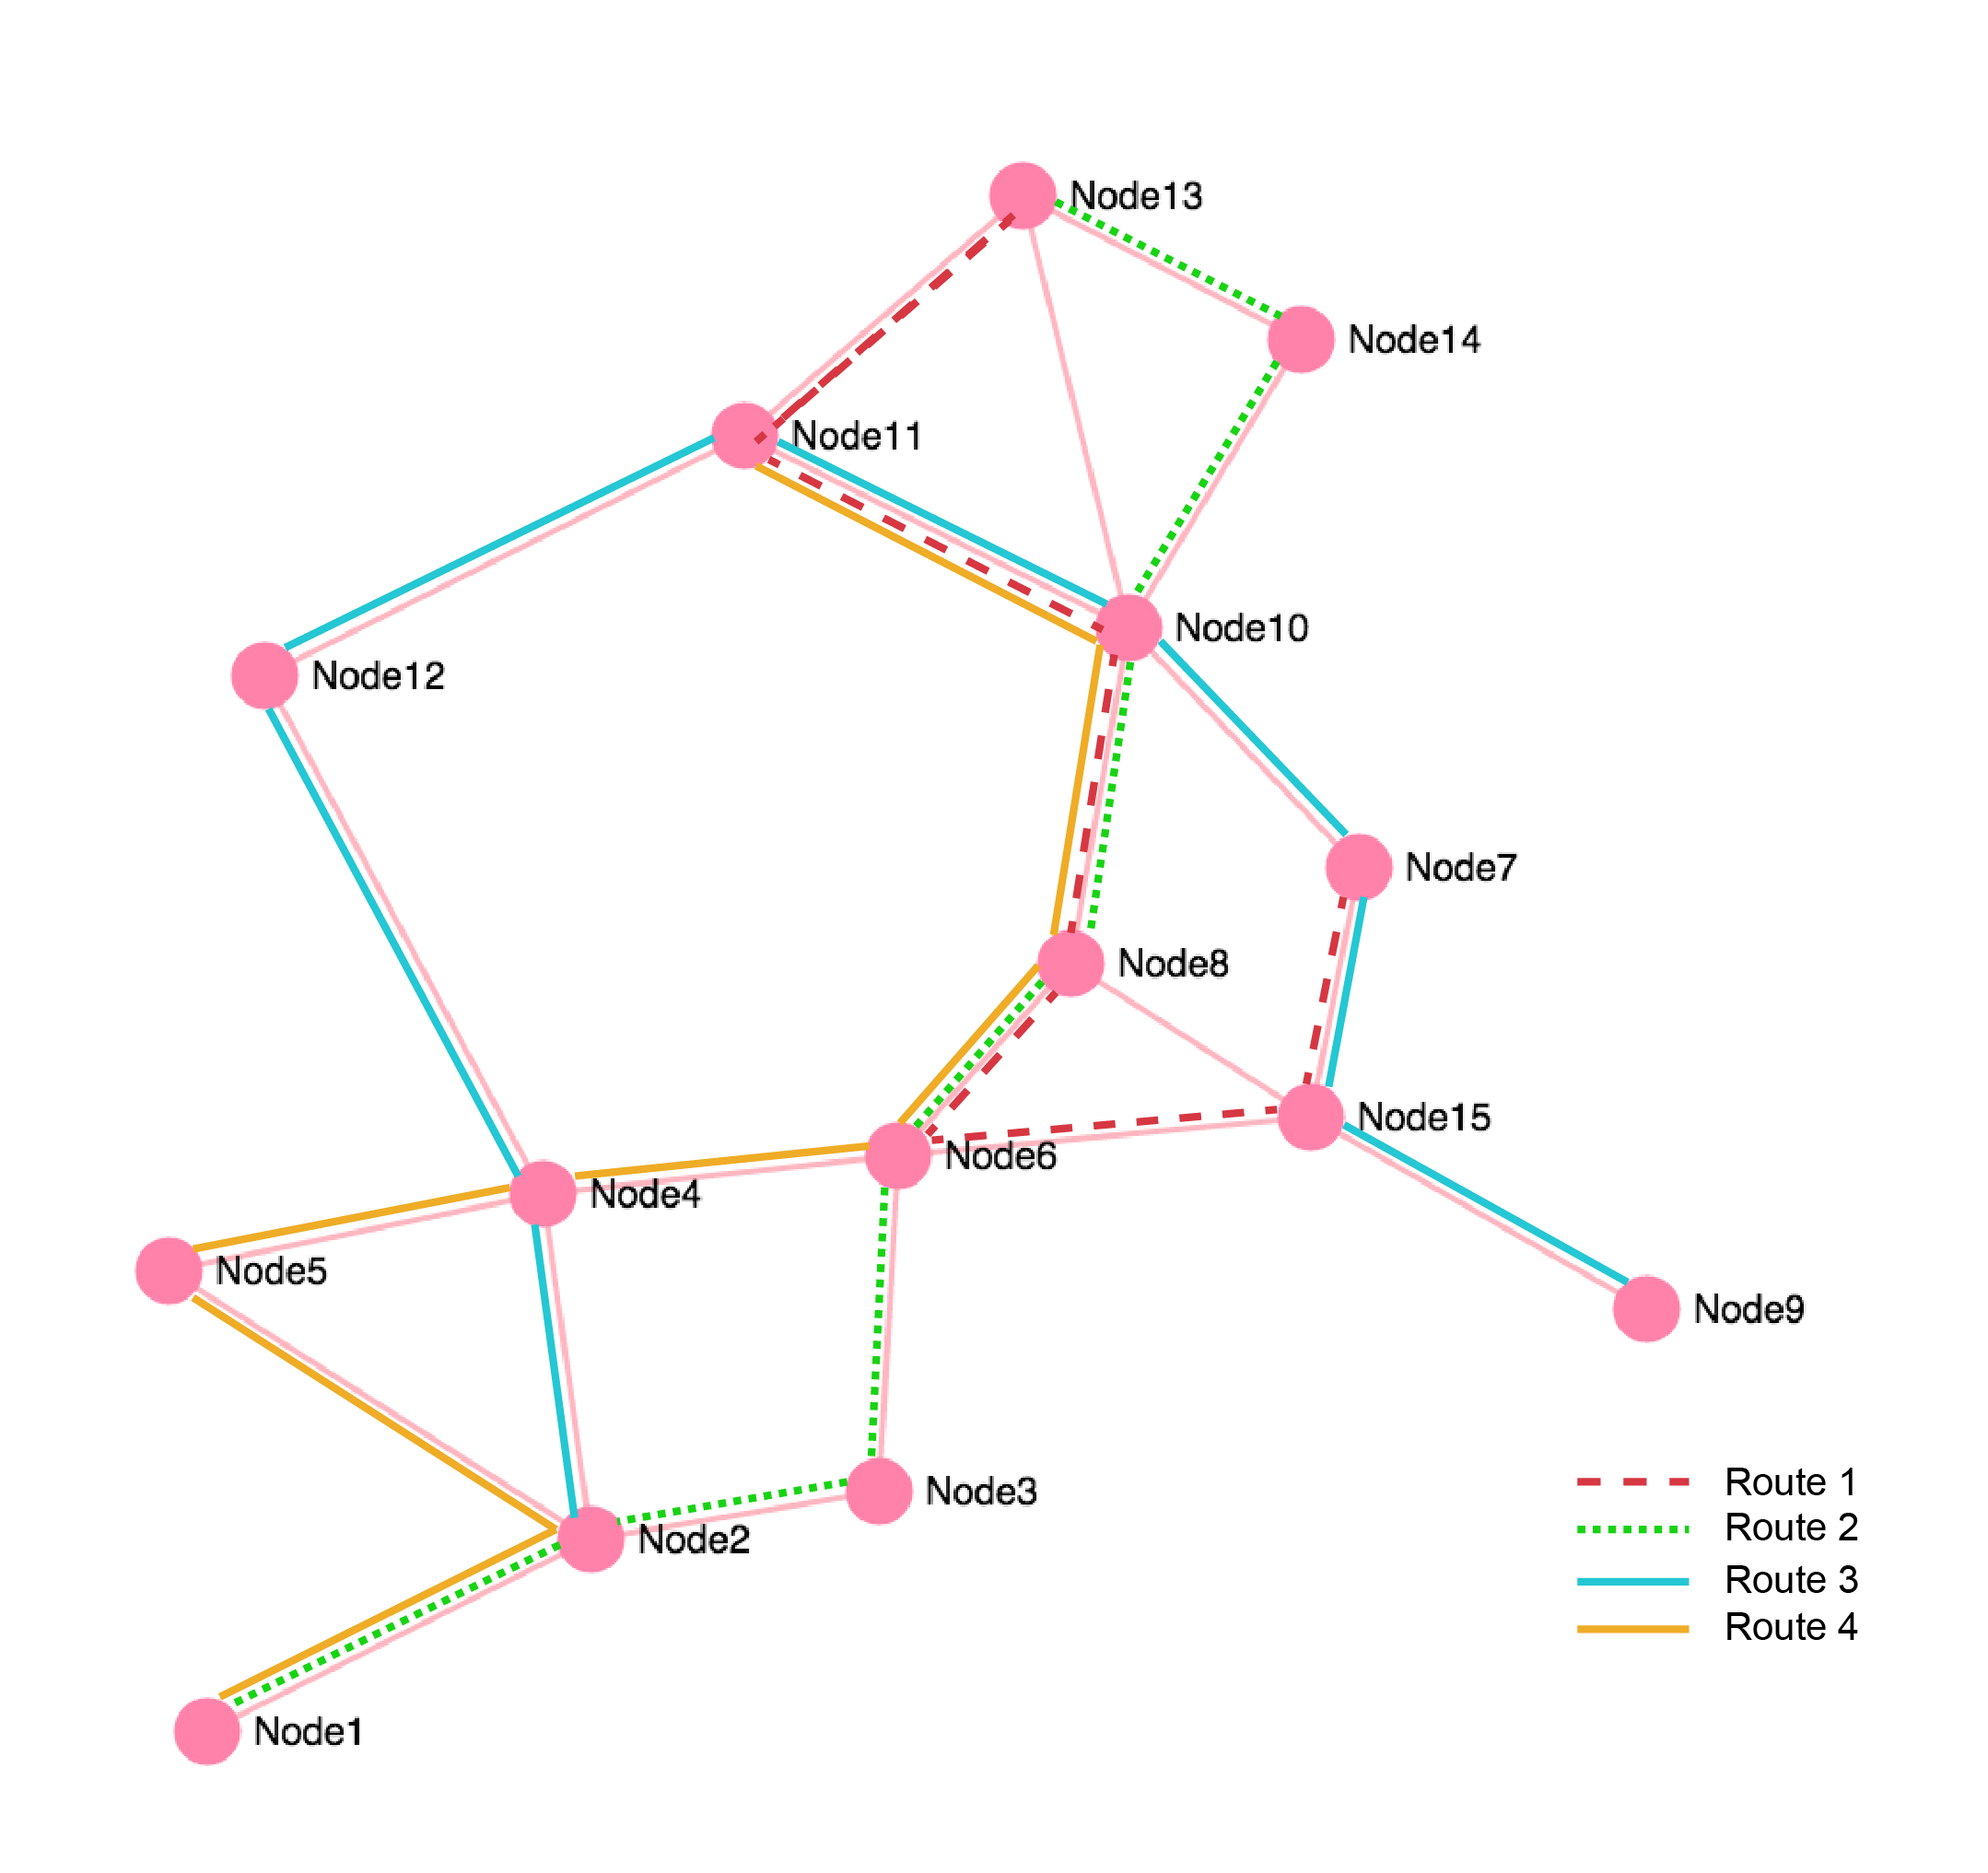
\includegraphics[width=4in]{assets/mandlnetwork_4routes.png}
  \end{center}
  \caption{Illustration of the best route set, having four routes, constructed by the proposed algorithm (Mandl's transit network as a graph)}
  \label{fig:bestRouteSet4} 
   %The transit network including the 15 nodes and 21 edges. The graph is undirected. \emph{\color{blue} TODO: Assumptions that it is undirected} Coordinates are correct based on the MandlCoordinates.txt file from \citep{mumford13}
\end{figure}


%-------------------- 6 route sets ---------------------

    \begin{table}[H]
    \centering
    \begin{tabular}{|l|l l l l l l l l|}
    \hline
    Route 1: & ~ & ~ & ~ & ~ & ~ & ~ & ~ & ~ \\
    Route 2: & ~ & ~ & ~ & ~ & ~ & ~ & ~ & ~ \\
    Route 3: & ~ & ~ & ~ & ~ & ~ & ~ & ~ & ~ \\
    Route 4: & ~ & ~ & ~ & ~ & ~ & ~ & ~ & ~ \\
    Route 5: & ~ & ~ & ~ & ~ & ~ & ~ & ~ & ~ \\
    Route 6: & ~ & ~ & ~ & ~ & ~ & ~ & ~ & ~ \\
    \hline
    \end{tabular}
    \caption {The best route set, having six routes}
    \label{table:performanceComparison_bestRouteSet6}
    \end{table}

    \begin{table}[H]
    \centering
    %\hspace*{-2.0cm}
    \begin{tabular}{|l||l|l|l|l|l|}
    \hline
    Algorithm & $d_0(\%)$ & $d_1(\%)$ & $d_2(\%)$ & $d_{unsat}(\%)$ & $ATT$ \\
    \hline
    \citet{kechagiopoulos14} & 95.62 & 4.28 & 0.10 & 0.00 & 10.28 \\
    %Kechapocholous BEST [ref] & 91.84 & 7.64 & 0.51 & 0.00 & 10.64 \\
    \citet{nikolic14} & 94.34 & 5.65 & 0.00 & 0.00 & - \\
    \citet{kidwai98} & 77.92 & 19.62 & 2.40 & 0.00 & 10.78 \\
    %\citet{fan09} best & & & & &  \\
    \citet{fan09} Hill Climbing & 90.23 & 9.26 & 0.51 & 0.00 & 11.69 \\
    \citet{fan09} Simulated Annealing & 90.87 & 8.74 & 0.39 & 0.00 & 10.65 \\
    \citet{chakroborty02} & 86.04 & 13.96 & 0.00 & 0.00 & 10.30 \\
    \citet{zhang10} & 91.12 & 8.88 & 0.00 & 0.00 & 10.50 \\
    \citet{chew12} & 93.85 & 5.88 & 0.24 & 0.03 & 10.51 \\
    \citet{baaj91} & 78.61 & 21.39 & 0.00 & 0.00 & 11.86 \\
    \hline
    \hline
    SSO Best & ~ & ~ & ~ & ~ & ~ \\
    SSO Average & ~ & ~ & ~ & ~ & ~ \\
    SSO Median & ~ & ~ & ~ & ~ & ~ \\
    SSO Worst & ~ & ~ & ~ & ~ & ~ \\
    SSO Standard Deviation & ~ & ~ & ~ & ~ & ~ \\
    SSO Relative Standard Deviation & ~ & ~ & ~ & ~ & ~ \\
    \hline
    \end{tabular}
    \caption {Comparing the best route set, having six routes}
    Results constructed by the proposed algorithm with average results published by other researchers.
    \label{table:performanceComparison_6}
    \end{table}

%-------------------- 7 route sets ---------------------

\begin{table}[H]
    \centering
    \begin{tabular}{|l|l l l l l l l l|}
    \hline
    Route 1: & ~ & ~ & ~ & ~ & ~ & ~ & ~ & ~ \\
    Route 2: & ~ & ~ & ~ & ~ & ~ & ~ & ~ & ~ \\
    Route 3: & ~ & ~ & ~ & ~ & ~ & ~ & ~ & ~ \\
    Route 4: & ~ & ~ & ~ & ~ & ~ & ~ & ~ & ~ \\
    Route 5: & ~ & ~ & ~ & ~ & ~ & ~ & ~ & ~ \\
    Route 6: & ~ & ~ & ~ & ~ & ~ & ~ & ~ & ~ \\
    Route 7: & ~ & ~ & ~ & ~ & ~ & ~ & ~ & ~ \\
    \hline
    \end{tabular}
    \caption {The best route set, having seven routes}
    \label{table:performanceComparison_bestRouteSet7}
    \end{table}

    \begin{table}[H]
    \centering
    %\hspace*{-2.0cm}
    \begin{tabular}{|l||l|l|l|l|l|}
    \hline
    Algorithm & $d_0(\%)$ & $d_1(\%)$ & $d_2(\%)$ & $d_{unsat}(\%)$ & $ATT$ \\
    \hline
    \citet{kechagiopoulos14} & 96.55 & 3.45 & 0.01 & 0.00 & 10.23 \\
    %Kechapocholous BEST [ref] & 91.84 & 7.64 & 0.51 & 0.00 & 10.64 \\
    \citet{nikolic14} & 94.41 & 5.59 & 0.00 & 0.00 & - \\
    \citet{kidwai98} & 93.91 & 6.09 & 0.00 & 0.00 & 10.70 \\
    %\citet{fan09} best & & & & &  \\
    \citet{fan09} Hill Climbing & 92.21 & 7.13 & 0.66 & 0.00 & 10.74 \\
    \citet{fan09} Simulated Annealing & 92.47 & 6.95 & 0.58 & 0.00 & 10.62 \\
    \citet{chakroborty02} & 89.15 & 10.85 & 0.00 & 0.00 & 10.15 \\
    \citet{zhang10} & 92.89 & 7.11 & 0.00 & 0.00 & 10.46 \\
    \citet{chew12} & 96.47 & 3.53 & 0.00 & 0.09 & 10.31 \\
    \citet{baaj91} & 80.99 & 19.01 & 0.00 & 0.00 & 12.50 \\
    \hline
    \hline
    SSO Best & ~ & ~ & ~ & ~ & ~ \\
    SSO Average & ~ & ~ & ~ & ~ & ~ \\
    SSO Median & ~ & ~ & ~ & ~ & ~ \\
    SSO Worst & ~ & ~ & ~ & ~ & ~ \\
    SSO Standard Deviation & ~ & ~ & ~ & ~ & ~ \\
    SSO Relative Standard Deviation & ~ & ~ & ~ & ~ & ~ \\
    \hline
    \end{tabular}
    \caption {Comparing the best route set, having seven routes}
    Results constructed by the proposed algorithm with average results published by other researchers.
    \label{table:performanceComparison_7}
    \end{table}
%-------------------- 8 route sets ---------------------

\begin{table}[H]
    \centering
    \begin{tabular}{|l|l l l l l l l l|}
    \hline
    Route 1: & ~ & ~ & ~ & ~ & ~ & ~ & ~ & ~ \\
    Route 2: & ~ & ~ & ~ & ~ & ~ & ~ & ~ & ~ \\
    Route 3: & ~ & ~ & ~ & ~ & ~ & ~ & ~ & ~ \\
    Route 4: & ~ & ~ & ~ & ~ & ~ & ~ & ~ & ~ \\
    Route 5: & ~ & ~ & ~ & ~ & ~ & ~ & ~ & ~ \\
    Route 6: & ~ & ~ & ~ & ~ & ~ & ~ & ~ & ~ \\
    Route 7: & ~ & ~ & ~ & ~ & ~ & ~ & ~ & ~ \\
    Route 8: & ~ & ~ & ~ & ~ & ~ & ~ & ~ & ~ \\
    \hline
    \end{tabular}
    \caption {The best route set, having eight routes}
    \label{table:performanceComparison_bestRouteSet8}
    \end{table}

    \begin{table}[H]
    \centering
    %\hspace*{-2.0cm}
    \begin{tabular}{|l||l|l|l|l|l|}
    \hline
    Algorithm & $d_0(\%)$ & $d_1(\%)$ & $d_2(\%)$ & $d_{unsat}(\%)$ & $ATT$ \\
    \hline
    \citet{kechagiopoulos14} avg & 97.47 & 2.53 & 0.00 & 0.00 & 10.17 \\
    %Kechapocholous BEST [ref] & 91.84 & 7.64 & 0.51 & 0.00 & 10.64 \\
    \citet{nikolic14} & 96.40 & 3.60 & 0.00 & 0.00 & - \\
    \citet{kidwai98} & 84.73 & 15.27 & 0.00 & 0.00 & 12.22 \\
    %\citet{fan09} best & & & & &  \\
    \citet{fan09} Hill Climbing & 93.23 & 6.18 & 0.59 & 0.00 & 10.69 \\
    \citet{fan09} Simulated Annealing & 93.65 & 5.88 & 0.47 & 0.00 & 10.58 \\
    \citet{chakroborty02} & 90.38 & 9.58 & 0.00 & 0.00 & 10.46 \\
    \citet{zhang10} & 93.14 & 6.86 & 0.00 & 0.00 & 10.42 \\
    \citet{chew12} & 96.16 & 3.84 & 0.00 & 0.09 & 10.31 \\
    \citet{baaj91} & 79.96 & 20.04 & 0.00 & 0.00 & 11.86 \\
    \hline
    \hline
    SSO Best & ~ & ~ & ~ & ~ & ~ \\
    SSO Average & ~ & ~ & ~ & ~ & ~ \\
    SSO Median & ~ & ~ & ~ & ~ & ~ \\
    SSO Worst & ~ & ~ & ~ & ~ & ~ \\
    SSO Standard Deviation & ~ & ~ & ~ & ~ & ~ \\
    SSO Relative Standard Deviation & ~ & ~ & ~ & ~ & ~ \\
    \hline
    \end{tabular}
    \caption {Comparing the best route set, having eight routes}
    Results constructed by the proposed algorithm with average results published by other researchers.
    \label{table:performanceComparison_8}
    \end{table}

\subsection{Scalability Experiments}
\label{subsec:scalabilityExperiments_results}
Grafer and stuff